\documentclass{article}[18pt]
\ProvidesPackage{format}
%Page setup
\usepackage[utf8]{inputenc}
\usepackage[margin=0.7in]{geometry}
\usepackage{parselines} 
\usepackage[english]{babel}
\usepackage{fancyhdr}
\usepackage{titlesec}
\hyphenpenalty=10000

\pagestyle{fancy}
\fancyhf{}
\rhead{Sam Robbins}
\rfoot{Page \thepage}

%Characters
\usepackage{amsmath}
\usepackage{amssymb}
\usepackage{gensymb}
\newcommand{\R}{\mathbb{R}}

%Diagrams
\usepackage{pgfplots}
\usepackage{graphicx}
\usepackage{tabularx}
\usepackage{relsize}
\pgfplotsset{width=10cm,compat=1.9}
\usepackage{float}

%Length Setting
\titlespacing\section{0pt}{14pt plus 4pt minus 2pt}{0pt plus 2pt minus 2pt}
\newlength\tindent
\setlength{\tindent}{\parindent}
\setlength{\parindent}{0pt}
\renewcommand{\indent}{\hspace*{\tindent}}

%Programming Font
\usepackage{courier}
\usepackage{listings}
\usepackage{pxfonts}

%Lists
\usepackage{enumerate}
\usepackage{enumitem}

% Networks Macro
\usepackage{tikz}


% Commands for files converted using pandoc
\providecommand{\tightlist}{%
	\setlength{\itemsep}{0pt}\setlength{\parskip}{0pt}}
\usepackage{hyperref}

% Get nice commands for floor and ceil
\usepackage{mathtools}
\DeclarePairedDelimiter{\ceil}{\lceil}{\rceil}
\DeclarePairedDelimiter{\floor}{\lfloor}{\rfloor}

% Allow itemize to go up to 20 levels deep (just change the number if you need more you madman)
\usepackage{enumitem}
\setlistdepth{20}
\renewlist{itemize}{itemize}{20}

% initially, use dots for all levels
\setlist[itemize]{label=$\cdot$}

% customize the first 3 levels
\setlist[itemize,1]{label=\textbullet}
\setlist[itemize,2]{label=--}
\setlist[itemize,3]{label=*}

% Definition and Important Stuff
% Important stuff
\usepackage[framemethod=TikZ]{mdframed}

\newcounter{theo}[section]\setcounter{theo}{0}
\renewcommand{\thetheo}{\arabic{section}.\arabic{theo}}
\newenvironment{important}[1][]{%
	\refstepcounter{theo}%
	\ifstrempty{#1}%
	{\mdfsetup{%
			frametitle={%
				\tikz[baseline=(current bounding box.east),outer sep=0pt]
				\node[anchor=east,rectangle,fill=red!50]
				{\strut Important};}}
	}%
	{\mdfsetup{%
			frametitle={%
				\tikz[baseline=(current bounding box.east),outer sep=0pt]
				\node[anchor=east,rectangle,fill=red!50]
				{\strut Important:~#1};}}%
	}%
	\mdfsetup{innertopmargin=10pt,linecolor=red!50,%
		linewidth=2pt,topline=true,%
		frametitleaboveskip=\dimexpr-\ht\strutbox\relax
	}
	\begin{mdframed}[]\relax%
		\centering
		}{\end{mdframed}}



\newcounter{lem}[section]\setcounter{lem}{0}
\renewcommand{\thelem}{\arabic{section}.\arabic{lem}}
\newenvironment{defin}[1][]{%
	\refstepcounter{lem}%
	\ifstrempty{#1}%
	{\mdfsetup{%
			frametitle={%
				\tikz[baseline=(current bounding box.east),outer sep=0pt]
				\node[anchor=east,rectangle,fill=blue!20]
				{\strut Definition};}}
	}%
	{\mdfsetup{%
			frametitle={%
				\tikz[baseline=(current bounding box.east),outer sep=0pt]
				\node[anchor=east,rectangle,fill=blue!20]
				{\strut Definition:~#1};}}%
	}%
	\mdfsetup{innertopmargin=10pt,linecolor=blue!20,%
		linewidth=2pt,topline=true,%
		frametitleaboveskip=\dimexpr-\ht\strutbox\relax
	}
	\begin{mdframed}[]\relax%
		\centering
		}{\end{mdframed}}
\lhead{MCS - DMLA}


\begin{document}
\begin{center}
\underline{\huge Linear Maps}
\end{center}
\section{Linear Maps}
\subsection{Definition}
Let V and W be vector spaces. A function $f: V\rightarrow W$ is called a linear map, or a linear transformation from V to W if, for all $u,v\in V, k\in \mathbb{R}$
$$f ( \mathbf { u } + \mathbf { v } ) = f ( \mathbf { u } ) + f ( \mathbf { v } ) \text { and } f ( k \mathbf { u } ) = k \cdot f ( \mathbf { u } )$$
If V=W then f is called a linear operator
\subsection{Examples}
\begin{itemize}
	\item The map $f:V\rightarrow W$ such that $f(u)=0$ for all u is linear
	\item If A is an $m\times n$ matrix then the map $f_A:\mathbb{R}^n\rightarrow \mathbb{R}^m$ given by $f_A(x)=Ax$ is linear. (Here x and Ax are column vectors in $\mathbb{R}^n$ and $\mathbb{R}^m$, respectively)\\
	Indeed,
	$$f _ { A } ( \mathbf { u } + \mathbf { v } ) = A ( \mathbf { u } + \mathbf { v } ) = A \mathbf { u } + A \mathbf { v } = f _ { A } ( \mathbf { u } ) + f _ { A } ( \mathbf { v } )$$
	and
	$$f _ { A } ( k \mathbf { u } ) = A ( k \mathbf { u } ) = k ( A \mathbf { u } ) = k f _ { A } ( \mathbf { u } )$$
\end{itemize}
\section{Non-examples in $\mathbb{R}^2$}
\begin{itemize}
	\item The map $g: \mathbb{R}^2\rightarrow \mathbb{R}^2$ defined by $g(x,y)=(x,y+1)$ is not linear . Indeed, any linear map f satisfies
	$$f ( \mathbf { 0 } ) = f ( 0 \mathbf { x } ) = 0 f ( \mathbf { x } ) = \mathbf { 0 }$$
	and the above map g fails this property
	\item The map $f: \mathbb{R}^2\rightarrow \mathbb{R}^2$ defined by $f(x,y)=(0,xy)$ is not linear. Indeed,
	$$f(e_1+e_2)=f(1,1)=(0,1)$$
	while
	$$f(e_1)+f(e_2)=f(0,1)+f(1,0)=(0,0)$$
\end{itemize}
\section{Example in $\mathbb{R}^2$}
\subsection{Reflection}
Consider linear operators $f_A$ on $\mathbb{R}^2$ where A is one of the following matrices
$$\left( \begin{array} { r r } { - 1 } & { 0 } \\ { 0 } & { 1 } \end{array} \right) , \quad \left( \begin{array} { r r } { 1 } & { 0 } \\ { 0 } & { - 1 } \end{array} \right) , \quad \left( \begin{array} { l l } { 0 } & { 1 } \\ { 1 } & { 0 } \end{array} \right)$$
The corresponding linear maps $f_A$ satisfy
$$f _ { A } ( x , y ) = ( - x , y ) , f _ { A } ( x , y ) = ( x , - y ) , f _ { A } ( x , y ) = ( y , x ) ,\text{respectively}$$
They correspond to \textbf{reflections} of $\mathbb{R}^2$ about the y-axis. x-axis, and line $x=y$ respectively
\begin{center}
	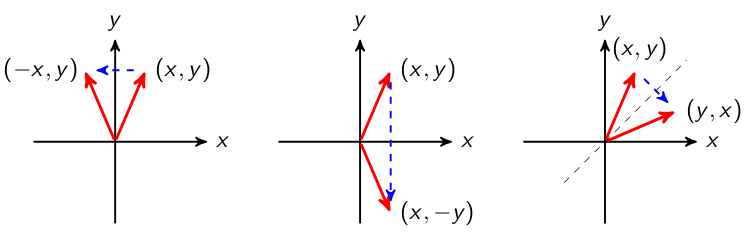
\includegraphics[scale=0.7]{reflections}
\end{center}
\subsection{Orthogonal Projection}
Consider linear operators $f_A$ on $\mathbb{R}^2$ where A is one of the following matrices
$$\left( \begin{array} { l l } { 1 } & { 0 } \\ { 0 } & { 0 } \end{array} \right) , \quad \left( \begin{array} { l l } { 0 } & { 0 } \\ { 0 } & { 1 } \end{array} \right)$$
The corresponding linear maps $f_A$ satisfy
\begin{center}
	$f _ { A } ( x , y ) = ( x , 0 )$ and $f _ { A } ( x , y ) = ( 0 , y ) ,$ respectively.
\end{center}
They correspond to the orthogonal projections of $\mathbb{R}^2$ onto x-axis and y-axis respectively
\begin{center}
	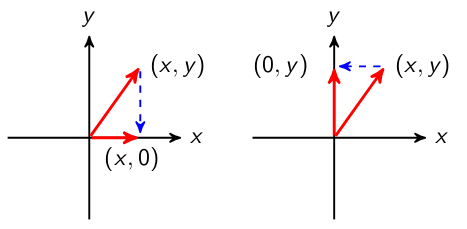
\includegraphics[scale=0.7]{projections}
\end{center}
 \subsection{Rotation}
 Consider the linear operator $f_A$ on $\mathbb{R}^2$ where A is the following matrix:
 $$\left( \begin{array} { c c } { \cos \theta } & { - \sin \theta } \\ { \sin \theta } & { \cos \theta } \end{array} \right)$$
 The corresponding linear map $f_A$ satisfies
 $$f _ { A } ( x , y ) = \left( x ^ { \prime } , y ^ { \prime } \right) = ( x \cos \theta - y \sin \theta , x \sin \theta + y \cos \theta )$$
This corresponds to the rotation of $\mathbb{R}^2$ by angle of $\theta$ counter clock-wise
\begin{center}
	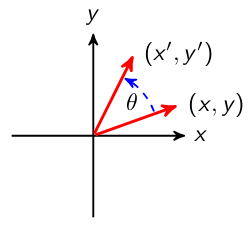
\includegraphics[scale=0.7]{rotation}
\end{center}
\subsection{Contraction/Dilation}
Consider linear operators $f_A$ on $\mathbb{R}^2$ where A is the following matrix
$$\left( \begin{array} { l l } { k } & { 0 } \\ { 0 } & { k } \end{array} \right)$$
The corresponding linear map $f_A$ satisfies
$$f _ { A } ( x , y ) = ( k x , k y )$$
This is \textbf{contraction} (if $0<k<1)$) or \textbf{dilation} (if $k>1$) of $\mathbb{R}^2$
\begin{center}
	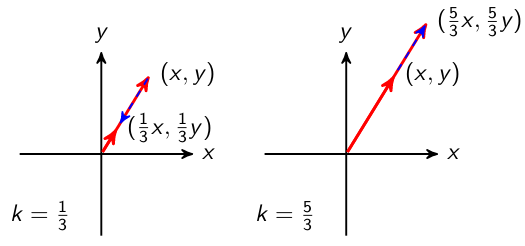
\includegraphics[scale=0.7]{contraction}
\end{center}
\subsection{Compression/Expansion}
Consider linear operators $f_A$ on $\mathbb{R}^2$ where A is one of the following matrices:
$$\left( \begin{array} { l l } { k } & { 0 } \\ { 0 } & { 1 } \end{array} \right) , \quad \left( \begin{array} { l l } { 1 } & { 0 } \\ { 0 } & { k } \end{array} \right)$$
The corresponding linear maps $f_A$ satisfy
\begin{center}
	$f _ { A } ( x , y ) = ( k x , y )$ and $f _ { A } ( x , y ) = ( x , k y ) ,$ respectively.
\end{center}
They correspond to \textbf{compressions} (if $0<k<1$) and \textbf{expansions} (if $k>1$) of $\mathbb{R}^2$ along x-axis and y-axis respectively
\begin{center}
	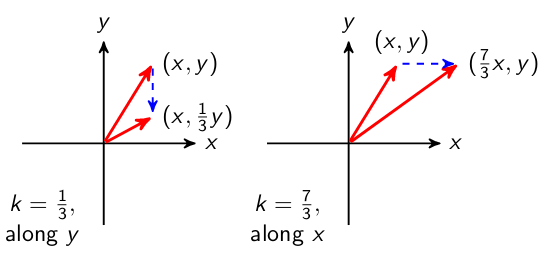
\includegraphics[scale=0.7]{compression}
\end{center}
\section{Bases and Linear Maps}
\subsection{Theorem}
Let $f:V\rightarrow W$ be a linear map where V is finite dimensional. If  $S = \left\{ \mathbf { v } _ { 1 } , \dots , \mathbf { v } _ { n } \right\}$ is a basis for V then the image of any vector $v\in V$ can be expressed as
$$f ( \mathbf { v } ) = c _ { 1 } f \left( \mathbf { v } _ { 1 } \right) + c _ { 2 } f \left( \mathbf { v } _ { 2 } \right) + \ldots + c _ { n } f \left( \mathbf { v } _ { n } \right)$$
where $c_1,...,c_n$ are the coordinates of v relative to S
\subsection{Proof}
Express $v \in V$ as $v = c _ { 1 } v _ { 1 } + c _ { 2 } v _ { 2 } + \dots + c _ { n } v _ { n }$ and use the linearity of $f$
\subsection{Theorem}
Conversely, if $f_0: S\rightarrow W$ is any map then the map $f:V\rightarrow W$ defined by
$$f ( \mathbf { v } ) = c _ { 1 } f _ { 0 } \left( \mathbf { v } _ { 1 } \right) + c _ { 2 } f _ { 0 } \left( \mathbf { v } _ { 2 } \right) + \ldots + c _ { n } f _ { 0 } \left( \mathbf { v } _ { n } \right)$$
where $c_1,...,c_n$ are the coordinates of v relative to S, is a linear map
\section{Exercise}
Consider the basis $S = \left\{ \mathbf { v } _ { 1 } , \mathbf { v } _ { 2 } , \mathbf { v } _ { 3 } \right\}$ in $\mathbb{R}^3$ where $v_1=(1,1,1), v_2=(1,1,0), v_3=(1,0,0)$ let $f: \mathbb{R}^3\rightarrow \mathbb{R}^3$ be a linear map such that
$$f \left( \mathbf { v } _ { 1 } \right) = ( 1,0 ) , f \left( \mathbf { v } _ { 2 } \right) = ( 2 , - 1 ) , f \left( \mathbf { v } _ { 3 } \right) = ( 4,3 )$$
Find a formula for $f(x_1,x_2,x_3)$ and use it to decide whether $f(2,-3,5)=(9,23)$
\subsection{Solution}
First express $x=(x_1,x_2,x_3)$ as $x=c_1v_1+c_2v_2+c_3v_3$ From this we get
$$\begin{aligned} c _ { 1 } + c _ { 2 } + c _ { 3 } & = x _ { 1 } \\ c _ { 1 } + c _ { 2 } & = x _ { 2 } \\ c _ { 1 } & = x _ { 3 } \end{aligned}$$
Which yields  $c _ { 1 } = x _ { 3 } , c _ { 2 } = x _ { 2 } - x _ { 3 } , c _ { 3 } = x _ { 1 } - x _ { 2 } ,$ so
$$\mathbf { x } = \left( x _ { 1 } , x _ { 2 } , x _ { 3 } \right) = x _ { 3 } \mathbf { v } _ { 1 } + \left( x _ { 2 } - x _ { 3 } \right) \mathbf { v } _ { 2 } + \left( x _ { 1 } - x _ { 2 } \right) \mathbf { v } _ { 3 }$$
Hence
$$f ( x ) = x _ { 3 } f \left( v _ { 1 } \right) + \left( x _ { 2 } - x _ { 3 } \right) f \left( v _ { 2 } \right) + \left( x _ { 1 } - x _ { 2 } \right) f \left( v _ { 3 } \right) = \left( 4 x _ { 1 } - 2 x _ { 2 } - x _ { 3 } , 3 x _ { 1 } - 4 x _ { 2 } + x _ { 3 } \right)$$
\section{The matrix of a linear map}
\begin{itemize}
	\item Let $f: \mathbb{R}^n\rightarrow \mathbb{R}^m$ be a linear map
	\item Let A be the $m\times n$ matrix $\left[ f \left( \mathbf { e } _ { 1 } \right) \left| f \left( \mathbf { e } _ { 2 } \right) \right| \ldots | f \left( \mathbf { e } _ { n } \right) \right]$ whose columns are vectors $f(e_i)\in \mathbb{R}^m$. For example, if $f:\mathbb{R}^3\rightarrow \mathbb{R}^2$ is linear and $f(1,0,0)=(2,3)$
	$$f ( 0,1,0 ) = ( 0,0 ) , f ( 0,0,1 ) = ( - 1,1 ) \text { then } A = \left( \begin{array} { c c c } { 2 } & { 0 } & { - 1 } \\ { 3 } & { 0 } & { 1 } \end{array} \right)$$
	\item Note that $f(e_i)=Ae_i=f_A(e_i)$ for all i, For example
	$$f \left( \mathbf { e } _ { 2 } \right) = \left( \begin{array} { c } { a _ { 12 } } \\ { a _ { 22 } } \\ { \vdots } \\ { a _ { m 2 } } \end{array} \right) = \left( \begin{array} { c c c c } { a _ { 11 } } & { a _ { 12 } } & { \cdots } & { a _ { 1 n } } \\ { a _ { 21 } } & { a _ { 22 } } & { \cdots } & { a _ { 2 n } } \\ { \vdots } & { \vdots } & { } & { \vdots } \\ { a _ { m 1 } } & { a _ { m 2 } } & { \cdots } & { a _ { m n } } \end{array} \right) \left( \begin{array} { c } { 0 } \\ { 1 } \\ { \vdots } \\ { 0 } \end{array} \right) = A \mathbf { e } _ { 2 } = f _ { A } \left( \mathbf { e } _ { 2 } \right)$$
	\item Since f and $f_A$ agree on all vectors in a basis, we have $f=f_A$
	\item Hence, every linear map $f:\mathbb{R}^n\rightarrow \mathbb{R}^m$ of the form $f_A$ for some matrix A
	\item This matrix A is called the (standard) matrix of linear map f
	\item Thus, linear maps from $\mathbb{R}^n$ to $\mathbb{R}^m$ are in 1-to-1 correspondence with $m\times n$ matrices (The same works for any pair of finite dimensional spaces)
\end{itemize}
\section{Exercise}
Find the standard matrix of the linear map $f:\mathbb{R}^4\rightarrow \mathbb{R}^3$ defined by
$$f \left( x _ { 1 } , x _ { 2 } , x _ { 3 } , x _ { 4 } \right) = \left( 7 x _ { 1 } + 2 x _ { 2 } - x _ { 3 } + x _ { 4 } , x _ { 2 } + x _ { 3 } , - x _ { 1 } \right)$$
\subsection{Solution}
We have
$$\begin{aligned} f ( 1,0,0,0 ) & = ( 7,0 , - 1 ) \\ f ( 0,1,0,0 ) & = ( 2,1,0 ) \\ f ( 0,0,1,0 ) & = ( - 1,1,0 ) \\ f ( 0,0,0,1 ) & = ( 1,0,0 ) \end{aligned}$$
Hence the matrix is
$$\left( \begin{array} { r r r r } { 7 } & { 2 } & { - 1 } & { 1 } \\ { 0 } & { 1 } & { 1 } & { 0 } \\ { - 1 } & { 0 } & { 0 } & { 0 } \end{array} \right)$$
\section{The kernel and range of a linear map}
\subsection{Definition}
Let $f: V\rightarrow W$ be a linear map\\
The \textbf{kernel} of f, denoted by $\operatorname{ker}(f)$ is defined by $\operatorname{ker}(f)=\{x\in V| f(x)=0\}$\\
The \textbf{range} of f  is defined as $\operatorname{range}( f ) = \{ \mathbf { u } \in W | \mathbf { u } = f ( \mathbf { x } ) \text { for some } \mathbf { x } \in V \}$
\begin{itemize}
	\item Let A be the standard matrix of a linear map $f : \mathbb { R } ^ { n } \rightarrow \mathbb { R } ^ { m } ( \text { so } f ( \mathbf { x } ) = A \mathbf { x } )$
	\item The $\operatorname{ker}(f)$ is the null space of A and $\operatorname{range}(f)$ is the column space of A
	\item Use algorithms for null space and column space to find $\operatorname{ker}(f)$ and $\operatorname{range}(f)$
\end{itemize}
\section{Dimension theorems for matrices and linear maps}
\subsection{Definition}
The \textbf{rank} of a linear map, denoted by rank(f), is the dimension of range(f)\\
The \textbf{nullity} of f, denoted by nullity(f), is the dimension of ker(f)\\
\\
Recall that, for a matrix A, rank(A) and nullity(A) are the dimensions of the column space and the null space of A. If A is the standard matrix of f then rank(A)=rank(f) and nullity(f)=nullity(A)
\subsection{Theorem (Dimension theorem for Matrices)}
For any matrix A with n columns, rank(A)+nullity(A)=n
\subsection{Theorem (Dimension Theorem for Linear Maps)}
If f is a linear map from $\mathbb{ R }^n$ to $\mathbb{ R }^m$ then rank(f)+nullity(f)=n
\section{Exercise}
If $f:\mathbb{ R }^5\rightarrow \mathbb{ R }^3$ is a linear map, what are the possible pairs (rank(f),nullity(f))?
\subsection{Solution}
$(0,5),(1,4),(2,3),(3,2)$. The pairs $(4,1)$ and $(5,0)$ are not possible because $\mathbb{ R }^3$ does not have a subspace of dimension $>3$
\end{document}